\documentclass[11pt,letterpaper]{article}
\usepackage[lmargin=1in,rmargin=1in,tmargin=1in,bmargin=1in]{geometry}
\usepackage{../style/homework}
\usepackage{../style/commands}
\setbool{quotetype}{false} % True: Side; False: Under
\setbool{hideans}{false} % Student: True; Instructor: False

% -------------------
% Content
% -------------------
\begin{document}

\homework{10: Due 11/05}{Our virtues and our  failures are inseparable, like force and matter. When they separate, man is no more.}{Nikola Tesla}

% Problem 1
\problem{10} Factor $x^2 + 7x - 30$. Show all your work. \pspace

\sol 
	\begin{table}[!ht]
	\centering
	\underline{\bfseries 30} \pvspace{0.2cm}
	\begin{tabular}{rr}
	$1 \cdot -30$ & $-29$ \\
	$-1 \cdot 30$ & $29$ \\
	$2 \cdot -15$ & $-13$ \\
	$-2 \cdot 15$ & $13$ \\
	$3 \cdot -10$ & $-7$ \\ \hline
	\multicolumn{1}{|r}{$-3 \cdot 10$} & \multicolumn{1}{r|}{$7$} \\ \hline
	$5 \cdot -6$ & $-1$ \\
	$-5 \cdot 6$ & $1$ 
	\end{tabular}
	\end{table}

Therefore,
	\[
	x^2 + 7x - 30= (x - 3)(x + 10)
	\]





\newpage





% Problem 2
\problem{10} Factor $x^2 - 12x + 36$. Show all your work. \pspace

\sol 
	\begin{table}[!ht]
	\centering
	\underline{\bfseries 36} \pvspace{0.2cm}
	\begin{tabular}{rr}
	$1 \cdot 36$ & $37$ \\
	$-1 \cdot -36$ & $-37$ \\
	$2 \cdot 18$ & $20$ \\
	$-2 \cdot -18$ & $-20$ \\
	$3 \cdot 12 $ & $15$ \\
	$-3 \cdot -12$ & $-15$ \\
	$4 \cdot 9$ & $13$ \\
	$-4 \cdot -9$ & $-13$ \\
	$6 \cdot 6$ & $12$ \\ \hline
	\multicolumn{1}{|r}{$-6 \cdot -6$} & \multicolumn{1}{r|}{$-12$} \\ \hline
	\end{tabular}
	\end{table}

Therefore,
	\[
	x^2 - 12x + 36= (x - 6)(x - 6)= (x - 6)^2
	\]





\newpage





% Problem 3
\problem{10} Factor $x^2 + 2x - 24$. Show all your work. \pspace

\sol 
	\begin{table}[!ht]
	\centering
	\underline{\bfseries 24} \pvspace{0.2cm}
	\begin{tabular}{rr}
	$1 \cdot -24$ & $-23$ \\
	$-1 \cdot 24$ & $23$ \\
	$2 \cdot -12$ & $-10$ \\
	$-2 \cdot 12$ & $10$ \\
	$3 \cdot -8 $ & $-5$ \\
	$-3 \cdot 8$ & $5$ \\
	$4 \cdot -6$ & $-2$ \\ \hline
	\multicolumn{1}{|r}{$-4 \cdot 6$} & \multicolumn{1}{r|}{$2$} \\ \hline
	\end{tabular}
	\end{table}

Therefore,
	\[
	x^2 + 2x - 24= (x - 4)(x + 6)
	\]





\newpage





% Problem 4
\problem{10} Factor $2x^2 + 9x - 18$. Show all your work. \pspace

\sol 
	\begin{table}[!ht]
	\centering
	\underline{\bfseries 18} \pvspace{0.1cm}
	\begin{tabular}{c}
	$1 \cdot -18$ \\
	$-1 \cdot 18$ \\
	$2 \cdot -9$ \\
	$-2 \cdot 9$ \\
	$3 \cdot -6$ \\
	$-3 \cdot 6$
	\end{tabular}
	\end{table}

Then as $2= 1 \cdot 2$, we have\dots
	\[
	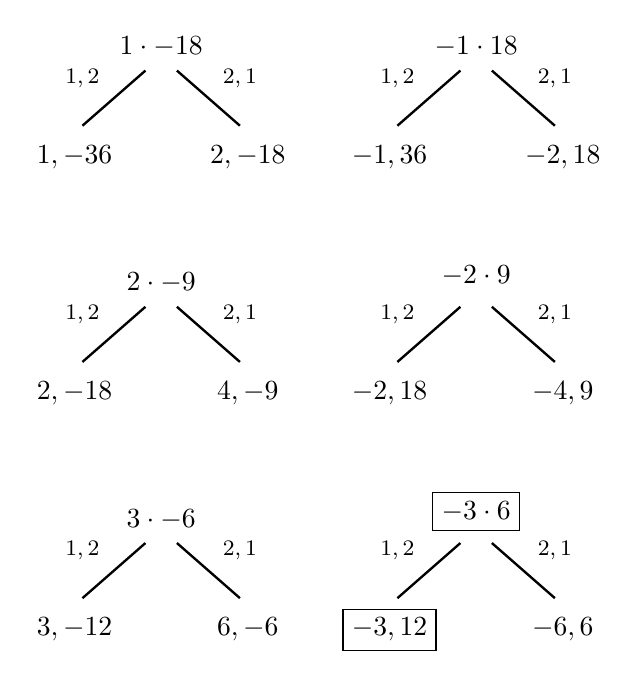
\begin{tikzpicture}
	\node at (0,0) {$1 \cdot -18$};
	\node at (-1.0,-0.4) {\footnotesize$1, 2$};
	\draw[line width=0.03cm,label={1}] (-0.2,-0.3) -- (-1,-1);
	\node at (-1.1,-1.4) {$1, -36$};
	\node at (1.0,-0.4) {\footnotesize$2,1$};
	\draw[line width=0.03cm] (0.2,-0.3) -- (1,-1);
	\node at (1.1,-1.4) {$2, -18$};	
	
	\tikzset{shift={(4,0)}}

	\node at (0,0) {$-1 \cdot 18$};
	\node at (-1.0,-0.4) {\footnotesize$1, 2$};
	\draw[line width=0.03cm,label={1}] (-0.2,-0.3) -- (-1,-1);
	\node at (-1.1,-1.4) {$-1, 36$};
	\node at (1.0,-0.4) {\footnotesize$2,1$};
	\draw[line width=0.03cm] (0.2,-0.3) -- (1,-1);
	\node at (1.1,-1.4) {$-2, 18$};

	\tikzset{shift={(-4,-3)}}

	\node at (0,0) {$2 \cdot -9$};
	\node at (-1.0,-0.4) {\footnotesize$1, 2$};
	\draw[line width=0.03cm,label={1}] (-0.2,-0.3) -- (-1,-1);
	\node at (-1.1,-1.4) {$2, -18$};
	\node at (1.0,-0.4) {\footnotesize$2,1$};
	\draw[line width=0.03cm] (0.2,-0.3) -- (1,-1);
	\node at (1.1,-1.4) {$4, -9$};

	\tikzset{shift={(4,0)}}

	\node at (0,0.1) {$-2 \cdot 9$};
	\node at (-1.0,-0.4) {\footnotesize$1, 2$};
	\draw[line width=0.03cm,label={1}] (-0.2,-0.3) -- (-1,-1);
	\node at (-1.1,-1.4) {$-2, 18$};
	\node at (1.0,-0.4) {\footnotesize$2,1$};
	\draw[line width=0.03cm] (0.2,-0.3) -- (1,-1);
	\node at (1.1,-1.4) {$-4, 9$};
	
	\tikzset{shift={(-4,-3)}}

	\node at (0,0) {$3 \cdot -6$};
	\node at (-1.0,-0.4) {\footnotesize$1, 2$};
	\draw[line width=0.03cm,label={1}] (-0.2,-0.3) -- (-1,-1);
	\node at (-1.1,-1.4) {$3, -12$};
	\node at (1.0,-0.4) {\footnotesize$2,1$};
	\draw[line width=0.03cm] (0.2,-0.3) -- (1,-1);
	\node at (1.1,-1.4) {$6, -6$};

	\tikzset{shift={(4,0)}}

	\node at (0,0.1) {\framebox{$-3 \cdot 6$}};
	\node at (-1.0,-0.4) {\footnotesize$1, 2$};
	\draw[line width=0.03cm,label={1}] (-0.2,-0.3) -- (-1,-1);
	\node at (-1.1,-1.4) {\framebox{$-3, 12$}};
	\node at (1.0,-0.4) {\footnotesize$2,1$};
	\draw[line width=0.03cm] (0.2,-0.3) -- (1,-1);
	\node at (1.1,-1.4) {$-6, 6$};
	\end{tikzpicture}
	\]

Therefore, 
	\[
	2x^2 + 9x - 18= (2x - 3)(x + 6)
	\]





\newpage





% Problem 5
\problem{10} Factor $18x^2 - 37x - 20$. Show all your work. \pspace

\sol
	\begin{table}[!ht]
	\centering
	\underline{\bfseries 20} \pvspace{0.1cm}
	\begin{tabular}{c}
	$1 \cdot -20$ \\
	$-1 \cdot 20$ \\
	$2 \cdot -10$ \\
	$-2 \cdot 10$ \\
	$4 \cdot -5$ \\
	$-4 \cdot 5$
	\end{tabular}
	\end{table}

Then as $18= 1 \cdot 18$, $18= 2 \cdot 9$, or $18= 3 \cdot 6$, we have\dots
	\[
	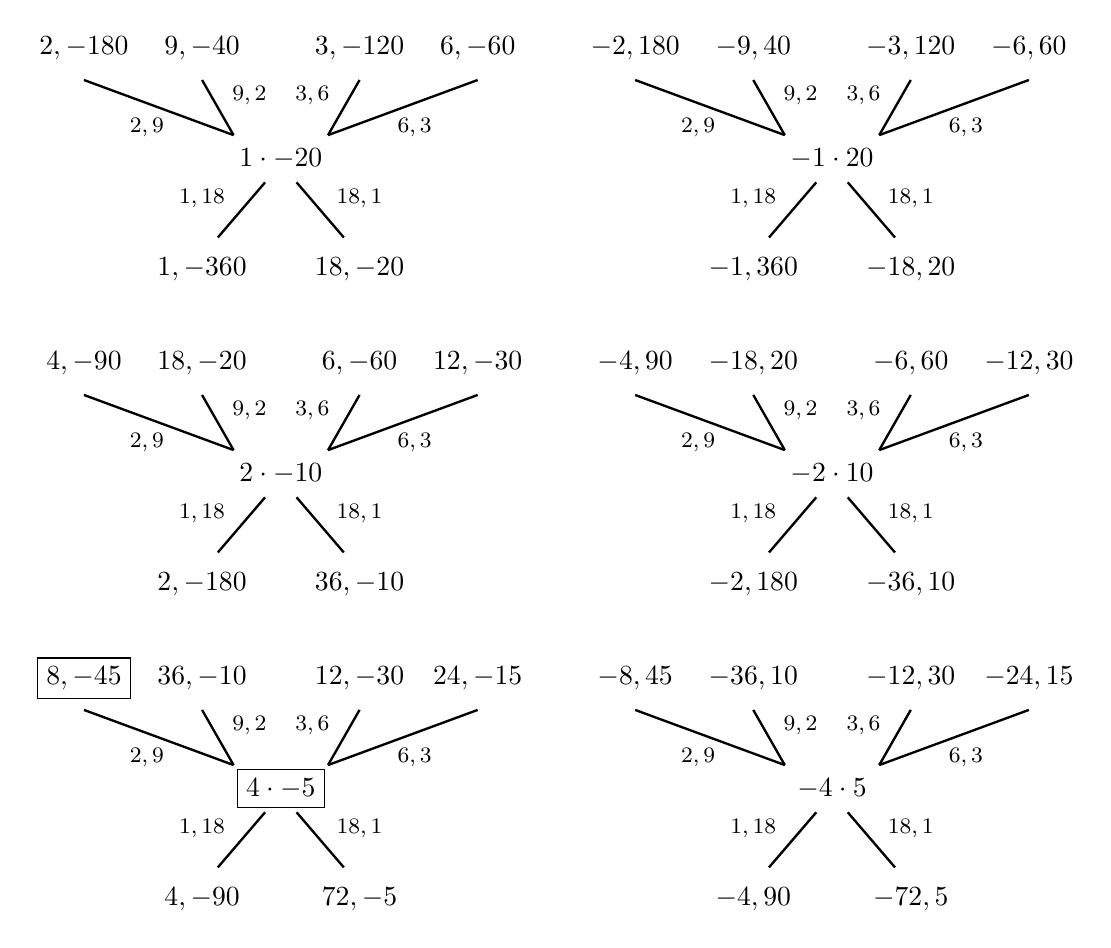
\begin{tikzpicture}
	\node at (0,0) {$1 \cdot -20$};
	
	\node at (-1.7,0.4) {\footnotesize$2, 9$};
	\draw[line width=0.03cm,label={1}] (-0.6,0.3) -- (-2.5,1);
	\node at (-2.5,1.4) {$2, -180$};
	
	\node at (-0.4,0.8) {\footnotesize$9, 2$};
	\draw[line width=0.03cm,label={1}] (-0.6,0.3) -- (-1,1);
	\node at (-1,1.4) {$9, -40$};

	\node at (0.4,0.8) {\footnotesize$3, 6$};
	\draw[line width=0.03cm,label={1}] (0.6,0.3) -- (1,1);
	\node at (1,1.4) {$3, -120$};
	
	\node at (1.7,0.4) {\footnotesize$6, 3$};
	\draw[line width=0.03cm,label={1}] (0.6,0.3) -- (2.5,1);
	\node at (2.5,1.4) {$6, -60$};
	
	\node at (-1,-0.5) {\footnotesize$1, 18$};
	\draw[line width=0.03cm,label={1}] (-0.2,-0.3) -- (-0.8,-1);
	\node at (-1,-1.4) {$1, -360$};

	\node at (1,-0.5) {\footnotesize$18, 1$};
	\draw[line width=0.03cm,label={1}] (0.2,-0.3) -- (0.8,-1);
	\node at (1,-1.4) {$18, -20$};

	\tikzset{shift={(7,0)}}
	
	\node at (0,0) {$-1 \cdot 20$};
	
	\node at (-1.7,0.4) {\footnotesize$2, 9$};
	\draw[line width=0.03cm,label={1}] (-0.6,0.3) -- (-2.5,1);
	\node at (-2.5,1.4) {$-2, 180$};
	
	\node at (-0.4,0.8) {\footnotesize$9, 2$};
	\draw[line width=0.03cm,label={1}] (-0.6,0.3) -- (-1,1);
	\node at (-1,1.4) {$-9, 40$};

	\node at (0.4,0.8) {\footnotesize$3, 6$};
	\draw[line width=0.03cm,label={1}] (0.6,0.3) -- (1,1);
	\node at (1,1.4) {$-3, 120$};
	
	\node at (1.7,0.4) {\footnotesize$6, 3$};
	\draw[line width=0.03cm,label={1}] (0.6,0.3) -- (2.5,1);
	\node at (2.5,1.4) {$-6, 60$};
	
	\node at (-1,-0.5) {\footnotesize$1, 18$};
	\draw[line width=0.03cm,label={1}] (-0.2,-0.3) -- (-0.8,-1);
	\node at (-1,-1.4) {$-1, 360$};

	\node at (1,-0.5) {\footnotesize$18, 1$};
	\draw[line width=0.03cm,label={1}] (0.2,-0.3) -- (0.8,-1);
	\node at (1,-1.4) {$-18, 20$};
	
	\tikzset{shift={(-7,-4)}}
	
	\node at (0,0) {$2 \cdot -10$};
	
	\node at (-1.7,0.4) {\footnotesize$2, 9$};
	\draw[line width=0.03cm,label={1}] (-0.6,0.3) -- (-2.5,1);
	\node at (-2.5,1.4) {$4, -90$};
	
	\node at (-0.4,0.8) {\footnotesize$9, 2$};
	\draw[line width=0.03cm,label={1}] (-0.6,0.3) -- (-1,1);
	\node at (-1,1.4) {$18, -20$};

	\node at (0.4,0.8) {\footnotesize$3, 6$};
	\draw[line width=0.03cm,label={1}] (0.6,0.3) -- (1,1);
	\node at (1,1.4) {$6, -60$};
	
	\node at (1.7,0.4) {\footnotesize$6, 3$};
	\draw[line width=0.03cm,label={1}] (0.6,0.3) -- (2.5,1);
	\node at (2.5,1.4) {$12, -30$};
	
	\node at (-1,-0.5) {\footnotesize$1, 18$};
	\draw[line width=0.03cm,label={1}] (-0.2,-0.3) -- (-0.8,-1);
	\node at (-1,-1.4) {$2, -180$};

	\node at (1,-0.5) {\footnotesize$18, 1$};
	\draw[line width=0.03cm,label={1}] (0.2,-0.3) -- (0.8,-1);
	\node at (1,-1.4) {$36, -10$};

	\tikzset{shift={(7,0)}}
	
	\node at (0,0) {$-2 \cdot 10$};
	
	\node at (-1.7,0.4) {\footnotesize$2, 9$};
	\draw[line width=0.03cm,label={1}] (-0.6,0.3) -- (-2.5,1);
	\node at (-2.5,1.4) {$-4, 90$};
	
	\node at (-0.4,0.8) {\footnotesize$9, 2$};
	\draw[line width=0.03cm,label={1}] (-0.6,0.3) -- (-1,1);
	\node at (-1,1.4) {$-18, 20$};

	\node at (0.4,0.8) {\footnotesize$3, 6$};
	\draw[line width=0.03cm,label={1}] (0.6,0.3) -- (1,1);
	\node at (1,1.4) {$-6, 60$};
	
	\node at (1.7,0.4) {\footnotesize$6, 3$};
	\draw[line width=0.03cm,label={1}] (0.6,0.3) -- (2.5,1);
	\node at (2.5,1.4) {$-12, 30$};
	
	\node at (-1,-0.5) {\footnotesize$1, 18$};
	\draw[line width=0.03cm,label={1}] (-0.2,-0.3) -- (-0.8,-1);
	\node at (-1,-1.4) {$-2, 180$};

	\node at (1,-0.5) {\footnotesize$18, 1$};
	\draw[line width=0.03cm,label={1}] (0.2,-0.3) -- (0.8,-1);
	\node at (1,-1.4) {$-36, 10$};
	
	\tikzset{shift={(-7,-4)}}
	
	\node at (0,0) {\framebox{$4 \cdot -5$}};
	
	\node at (-1.7,0.4) {\footnotesize$2, 9$};
	\draw[line width=0.03cm,label={1}] (-0.6,0.3) -- (-2.5,1);
	\node at (-2.5,1.4) {\framebox{$8, -45$}};
	
	\node at (-0.4,0.8) {\footnotesize$9, 2$};
	\draw[line width=0.03cm,label={1}] (-0.6,0.3) -- (-1,1);
	\node at (-1,1.4) {$36, -10$};

	\node at (0.4,0.8) {\footnotesize$3, 6$};
	\draw[line width=0.03cm,label={1}] (0.6,0.3) -- (1,1);
	\node at (1,1.4) {$12, -30$};
	
	\node at (1.7,0.4) {\footnotesize$6, 3$};
	\draw[line width=0.03cm,label={1}] (0.6,0.3) -- (2.5,1);
	\node at (2.5,1.4) {$24, -15$};
	
	\node at (-1,-0.5) {\footnotesize$1, 18$};
	\draw[line width=0.03cm,label={1}] (-0.2,-0.3) -- (-0.8,-1);
	\node at (-1,-1.4) {$4, -90$};

	\node at (1,-0.5) {\footnotesize$18, 1$};
	\draw[line width=0.03cm,label={1}] (0.2,-0.3) -- (0.8,-1);
	\node at (1,-1.4) {$72, -5$};

	\tikzset{shift={(7,0)}}
	
	\node at (0,0) {$-4 \cdot 5$};
	
	\node at (-1.7,0.4) {\footnotesize$2, 9$};
	\draw[line width=0.03cm,label={1}] (-0.6,0.3) -- (-2.5,1);
	\node at (-2.5,1.4) {$-8, 45$};
	
	\node at (-0.4,0.8) {\footnotesize$9, 2$};
	\draw[line width=0.03cm,label={1}] (-0.6,0.3) -- (-1,1);
	\node at (-1,1.4) {$-36, 10$};

	\node at (0.4,0.8) {\footnotesize$3, 6$};
	\draw[line width=0.03cm,label={1}] (0.6,0.3) -- (1,1);
	\node at (1,1.4) {$-12, 30$};
	
	\node at (1.7,0.4) {\footnotesize$6, 3$};
	\draw[line width=0.03cm,label={1}] (0.6,0.3) -- (2.5,1);
	\node at (2.5,1.4) {$-24, 15$};
	
	\node at (-1,-0.5) {\footnotesize$1, 18$};
	\draw[line width=0.03cm,label={1}] (-0.2,-0.3) -- (-0.8,-1);
	\node at (-1,-1.4) {$-4, 90$};

	\node at (1,-0.5) {\footnotesize$18, 1$};
	\draw[line width=0.03cm,label={1}] (0.2,-0.3) -- (0.8,-1);
	\node at (1,-1.4) {$-72, 5$};	
	\end{tikzpicture}
	\]

Therefore, 
	\[
	18x^2 - 37x - 20= (2x - 5)(9x + 4)
	\]


%\printpoints
\end{document}